\documentclass[simplex.tex]{subfiles}
% DO NOT INCLUDE PREAMBLES/PACKAGES HERE!!
% packages are inherited from preamble.tex; you can compile this on its own
\begin{document}
\subsection{FlashX}

We advance FlashR for exploratory analysis on a billion-scale
graph. This includes functions for filtering data points and plotting
histograms and heatmaps on billions of data points. Figure \ref{fig:FlashX}
shows an example of plotting the in-degree histogram of vertices in the page
graph and a heatmap for the distribution of the vertices of the page graph in
a two-dimension space.

\begin{figure}[!h]
\begin{cframed}
\centering
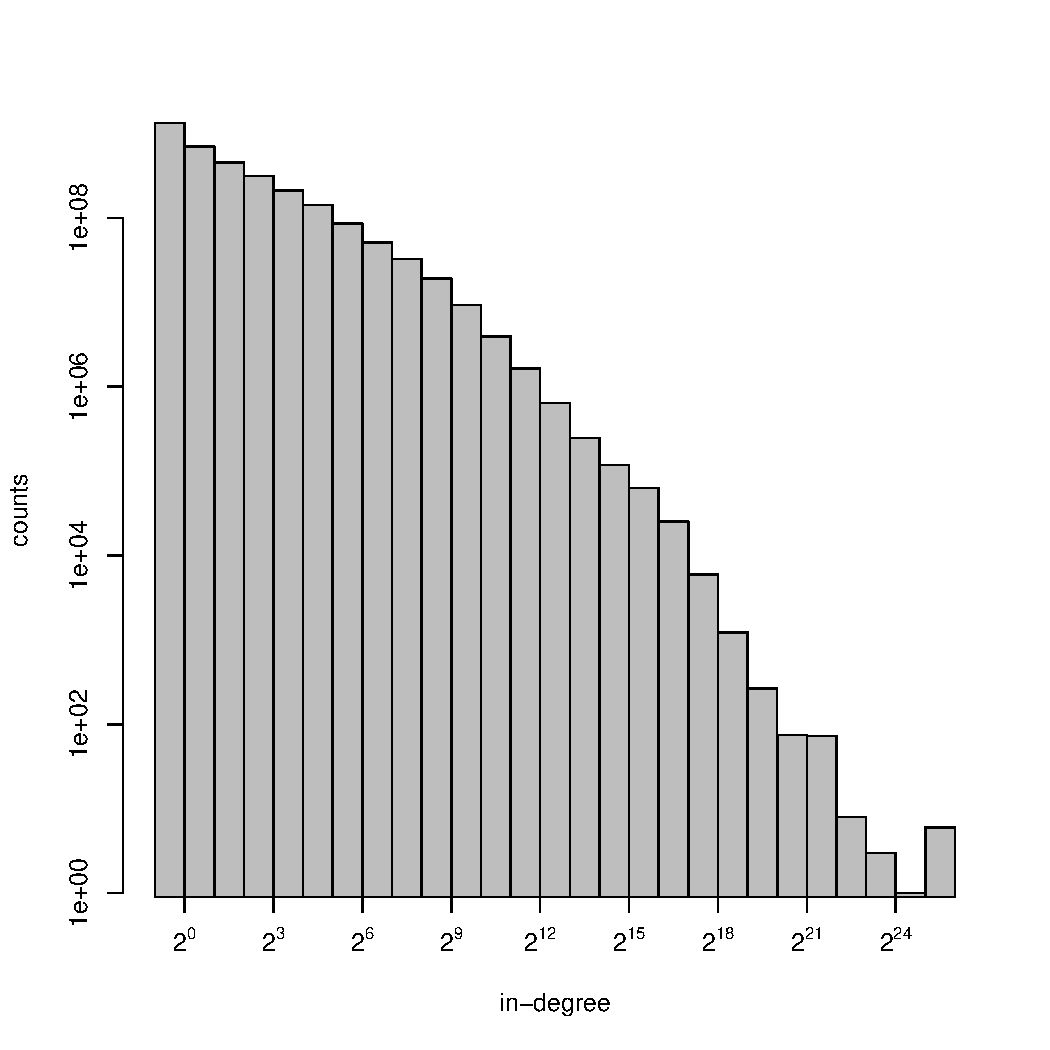
\includegraphics[width=0.4\textwidth]{../../figs/hist-indeg.pdf}
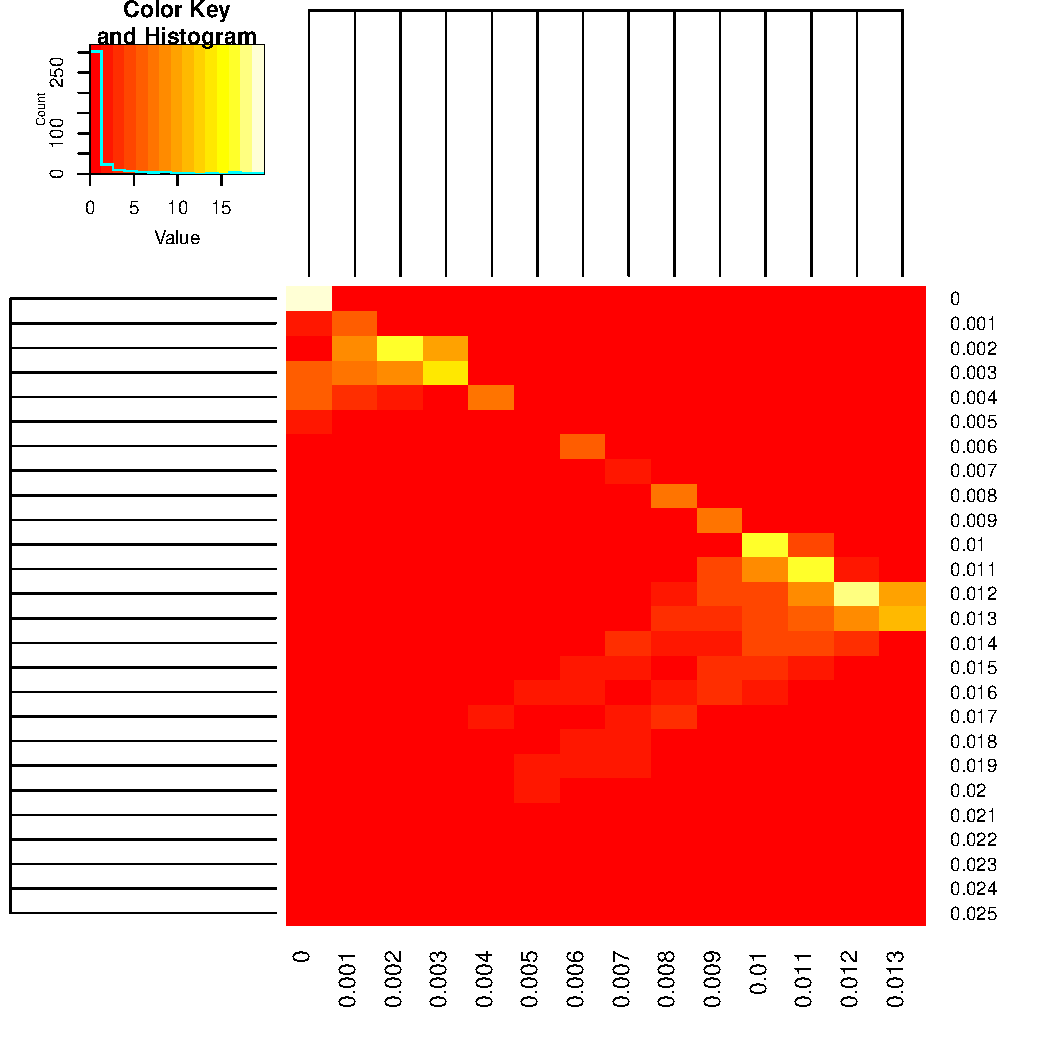
\includegraphics[width=0.4\textwidth]{../../figs/pg_xy_heatmap.pdf}
\caption{Left: the in-degree distribution of the Page graph.
	Right: a heatmap of the distribution of the vertices of the page graph
	in a two-dimension space; the coordinates of the vertices
	in the two-dimension space is determined by the first left and right
	singular vectors.}
\label{fig:FlashX}
\end{cframed}
\end{figure}

\clearpage
\end{document}
